%% Argos --- Mid-Term Progress Report
%% IEEE conference format (IEEEtran). First draft.
%%
%% This is a MID-TERM progress report, not the research paper.
%% Scope: problem framing, objectives, work-completed audit, preliminary
%% measurements, remaining work, timeline. Companion to paper_ieee.tex.

\documentclass[conference]{IEEEtran}
\IEEEoverridecommandlockouts

\usepackage{cite}
\usepackage{amsmath,amssymb,amsfonts}
\usepackage{graphicx}
\usepackage{xcolor}
\usepackage{booktabs}
\usepackage{url}
\usepackage{array}
\usepackage{hyperref}
\usepackage{tikz}
\usetikzlibrary{calc}
\hypersetup{colorlinks=true,linkcolor=blue!50!black,citecolor=blue!40!black,urlcolor=blue!50!black}

\begin{document}

\title{Argos --- A Multi-Agent LLM Trading Research Desk\\
\large Mid-Term Progress Report}

\author{
\IEEEauthorblockN{Kishor Timilsena}
\IEEEauthorblockA{Fuse-AI Fellowship\\
Department of Computer Science and Engineering\\
\textit{<home institution>}}
}

\maketitle

\begin{abstract}
This mid-term report documents the design, implementation, and
preliminary measurement of \emph{Argos}, a multi-agent Large
Language Model (LLM) trading research desk built as a Fuse-AI
fellowship project. We report (i) the completed pipeline: an
eight-node LangGraph orchestration of specialized agents
(fundamentals, sentiment, technicals, bull/bear debate, blind judge,
risk, portfolio manager) with a novel selective-reasoning gate;
(ii) the trader-facing research-desk front-end that pairs raw
evidence with each agent's structured verdict across five panels
(Fundamentals, Technicals, Sentiment, Ownership, Risk);
(iii) preliminary measurements across four NASDAQ tickers (NVDA,
TSLA, ORCL, KO) over 2024 ($n{=}211$ decisions) including per-agent
calibration, confidence asymmetry, and a cost--recall Pareto
frontier; and (iv) the remaining work plan through the project's
final milestone. 65\% of the planned deliverables are complete;
three deliverables remain (ablation completeness, out-of-sample
validation, and final paper submission). Projected completion date:
within the final milestone window.
\end{abstract}

\begin{IEEEkeywords}
mid-term report, multi-agent LLM, financial research desk,
selective prediction, calibration, LangGraph, project management
\end{IEEEkeywords}

%% =====================================================================
\section{Problem Statement and Objectives}

\subsection{Problem}
Multi-agent LLM systems have been proposed as the next step for
quantitative financial research~\cite{tradingagents,finagent,finmem},
but they share three measurement weaknesses: (i) per-decision token
cost is rarely reported, despite being the dominant operating
expense; (ii) the HOLD / abstain outcome dominates committee outputs
but the deliberation that produces it is unexamined;
(iii) per-agent contribution is not disaggregated, which makes
ablation claims unreliable. A reviewer cannot decide whether the
system's architecture carries signal or whether gains are explained
by data contamination, lucky baselines, or ticker-selection bias.

\subsection{Objectives}
The project sets five objectives:

\begin{enumerate}
  \item Build an eight-agent LLM pipeline with structured outputs,
  per-decision journaling, and reproducibility metadata (git SHA,
  pinned model IDs, cache hashes).
  \item Introduce a \emph{selective-reasoning gate} before the
  debate stage and measure its cost--recall--calibration tradeoff.
  \item Produce a \emph{research-desk front-end} that pairs raw
  numeric evidence with the structured verdict of the agent that
  reasoned over it, so the LLM committee is auditable panel-by-panel.
  \item Produce the \emph{ablation table family} CLAUDE.md names as
  required: gate on/off, judge on/off, debate rounds, Kronos
  live/stub, leave-one-analyst-out.
  \item Submit a measurement-first research paper to the Fuse-AI
  fellowship cycle.
\end{enumerate}

Objectives 1--3 are complete. Objective 4 is $\sim$60\% complete.
Objective 5 has a first-draft IEEE-format manuscript (companion to
this report).

%% =====================================================================
\section{Scope of Mid-Term Deliverable}

The mid-term delivery covers:
\begin{itemize}
  \item The full pipeline topology and all agent prompts (frozen).
  \item The reference run under
  \texttt{logs/decisions/nasdaq\_focus/} ($n{=}211$ weekly decisions
  across four tickers in 2024).
  \item The research-desk front-end (React + FastAPI) with the five
  two-layer panels, chart with decision-dot overlays, SSE live
  streaming of the committee, and a trust-layer Analytics view.
  \item The gate-on/gate-off ablation and the Pareto threshold
  sweep.
  \item The per-agent reliability analysis (Brier, ECE).
  \item The baseline comparison (buy-and-hold, moving-average
  cross, random, logistic learned-gate).
  \item The first-draft paper manuscript (IEEE format).
\end{itemize}

The final delivery will extend ablation coverage (judge, debate
rounds, Kronos, LOO analyst), add walk-forward out-of-sample
validation, and ship the final manuscript.

%% =====================================================================
\section{Related Work --- a Positioning Summary}

A fuller survey appears in the companion research paper. For the
purpose of the mid-term review the positioning is:

\textbf{Multi-agent LLM finance}~\cite{tradingagents,finagent,finmem}
proposes pipelines of specialized LLM agents for trading decisions.
These works report returns but do not report token cost per decision,
do not disaggregate per-agent calibration, and do not treat
abstention as a measured output.

\textbf{Selective prediction and learning-to-defer}~\cite{
chow1970,geifman2017selective,mozannar2020defer} formalize the
decision to abstain and trade coverage for accuracy. We extend this
family one level up --- our gate decides whether the \emph{downstream
multi-agent reasoning procedure} runs.

\textbf{Multi-agent debate}~\cite{du2023debate,liang2023divergent}
introduces adversarial debate as an LLM reasoning procedure. Our
bull--bear step adopts this; our contribution over this literature is
to measure confidence asymmetry under \emph{symmetric model routing}
(same model, key, prompt scaffold for both sides).

\textbf{LLM cost efficiency}~\cite{chen2023frugalgpt,ong2024routellm}
reduces per-inference cost by model substitution. Our gate is
complementary --- it reduces \emph{whether} the expensive path runs,
orthogonal to which model it uses.

%% =====================================================================
\section{Methodology --- What We Built}

\subsection{System topology}
Argos is a LangGraph~\cite{langgraph} pipeline of eight LLM-backed
nodes (Fig.~\ref{fig:topology}):
\texttt{exit\_manager} $\to$
\texttt{\{fundamentals, sentiment, technicals\}}$_{\text{parallel}}$
$\to$ \texttt{kronos\_forecast} $\to$ \texttt{edge\_gate} $\to$
\texttt{bull/bear debate} $\to$ \texttt{blind\_judge} $\to$
\texttt{risk\_manager} $\to$ \texttt{portfolio\_manager}. Two
short-circuit paths exist: exit-manager (when a position is open)
and gate (when the gate decides against convening the committee).

\begin{figure}[t]
\centering
\begin{tikzpicture}[
  node distance=1.5mm,
  box/.style={draw, rounded corners=1.5pt, align=center,
              font=\scriptsize, minimum height=5mm, minimum width=14mm,
              inner sep=1.2pt},
  gate/.style={draw, rounded corners=1.5pt, thick, align=center,
               font=\scriptsize\bfseries,
               minimum height=5mm, minimum width=14mm, inner sep=1.2pt,
               fill=yellow!15},
  arr/.style={-latex, thin}
]
\node[box] (start) {\texttt{START}};
\node[box, right=of start] (exit) {\texttt{exit\_mgr}};
\node[box, below=of exit] (fund) {\texttt{fund.}};
\node[box, below=of fund] (sent) {\texttt{sent.}};
\node[box, below=of sent] (tech) {\texttt{tech.}};
\node[box, right=of fund, xshift=3mm] (kronos) {\texttt{kronos}};
\node[gate, right=of kronos] (gate) {\texttt{edge\_gate}};
\node[box, below=of gate] (debate) {\texttt{bull/bear}};
\node[box, below=of debate] (judge) {\texttt{judge}};
\node[box, below=of judge] (risk) {\texttt{risk}};
\node[box, left=of risk] (pm) {\texttt{pm}};
\node[box, left=of pm] (end) {\texttt{END}};
\draw[arr] (start) -- (exit);
\draw[arr] (exit) -- (fund);
\draw[arr] (exit.east) -- ++(4mm,0) |- (end.east);
\draw[arr] (fund) -- (kronos);
\draw[arr] (sent.east) -| (kronos);
\draw[arr] (tech.east) -| (kronos);
\draw[arr] (kronos) -- (gate);
\draw[arr] (gate) -- (debate);
\draw[arr] (gate.east) -- ++(4mm,0) |- (end.east);
\draw[arr] (debate) -- (judge);
\draw[arr] (judge) -- (risk);
\draw[arr] (risk) -- (pm);
\draw[arr] (pm) -- (end);
\end{tikzpicture}
\caption{Argos pipeline. The selective-reasoning gate (bold, yellow)
is the primary research contribution. Exit-manager and gate are the
two short-circuit paths.}
\label{fig:topology}
\end{figure}

\subsection{Structured outputs and journal}
Every agent emits a Pydantic-validated structured output
(\texttt{AnalystSignal}, \texttt{DebateArgument}, \texttt{JudgeVerdict},
\texttt{RiskVerdict}, \texttt{FinalDecision}). Each decision is written
as one JSONL file at
\texttt{logs/decisions/<namespace>/<TICKER>/<TICKER>\_<YYYY-MM-DD>.jsonl}
including the exact prompt sent to each agent, each agent's
structured output, per-agent token counts, the gate verdict, the
indicator snapshot, and the git SHA that produced it.

\subsection{Selective-reasoning gate}
The gate is one additional structured LLM call (pinned to a cheap
model tier) that reads the analyst signals and the indicator snapshot
and emits \texttt{proceed}~$\in\{$True, False$\}$, a confidence, and
a list of triggers from a fixed vocabulary of eight symbols. The
gate's prompt is intentionally \emph{recall-biased}: when in doubt,
proceed. The design hypothesis to test is that aggressive
thresholding trades coverage for accuracy without destroying recall.

\subsection{Research-desk front-end}
A trader-facing React + Vite + TypeScript front-end backed by a
FastAPI service. Per-ticker screen has three bands:
(i) chart with candles, MA(20/50/200), RSI(14) sub-pane, and
decision-dot overlays colored by action and sized by confidence;
(ii) five two-layer panels --- raw evidence on top, structured
agent verdict below --- for Fundamentals, Technicals, Sentiment,
Ownership, Risk; (iii) a committee band with SSE-streamed
pipeline rail and final-decision strip. A separate Analytics view
exposes the calibration curve, abstention rates, and the override
log. Every verdict carries a stage badge
(\texttt{backtest}/\texttt{walk\_forward}/\texttt{paper}/\texttt{live})
so a reader can tell at a glance which trust tier produced it.

\subsection{Research framing}
Per CLAUDE.md the project is positioned \emph{research-first}: HOLD
is reported as a measured output (selective abstention), not an
absence of trade; every claim carries a sample size and uncertainty
band; no prompt change ships without a paired A/B ablation; all
model IDs are pinned (never \texttt{-latest}). This positioning
lives in the code via append-only JSONL journals,
\texttt{argos/token\_usage.py} per-decision accounting, and shared
ablation harness at \texttt{argos/reports/ablation.py}.

%% =====================================================================
\section{Preliminary Measurements}

\subsection{Headline portfolio numbers}
Paper account starting at \$1{,}000 per ticker. Across 2024
(Table~\ref{tab:portfolio}):

\begin{table}[t]
\caption{Paper portfolio returns per ticker, 2024.}
\label{tab:portfolio}
\centering\footnotesize
\begin{tabular}{lrrr}
\toprule
Ticker & Start cash & End equity & Return \\
\midrule
NVDA  & \$1{,}000.00 & \$1{,}018.38 & $+1.84\%$ \\
TSLA  & \$1{,}000.00 & \$1{,}000.00 & $0.00\%$ \\
ORCL  & \$1{,}000.00 & \$1{,}000.23 & $+0.02\%$ \\
KO    & \$1{,}000.00 & \$1{,}002.28 & $+0.23\%$ \\
\midrule
Total & \$4{,}000.00 & \$4{,}020.89 & $+0.52\%$ \\
\bottomrule
\end{tabular}
\end{table}

The system traded conservatively: 20\% of cash per position cap,
median one paper trade per ticker across the year. TSLA was not
traded at all --- the debate never converged. This is a measured
outcome of the design, not a bug: abstention is reported as a
first-class result in the companion paper.

\subsection{Pipeline cost}
Across the full $n{=}211$ weekly decisions:
\begin{itemize}
  \item $5\,601\,846$ total tokens
  \item $1\,461$ total LLM calls
  \item $\sim$26\,400 tokens per decision (dominant cost in debate,
  judge, risk, PM stages)
  \item $\sim$6.9 LLM calls per decision
  \item Realized API spend: \$6--\$8 over the 2024 reference run
\end{itemize}

\subsection{Directional accuracy}
The pipeline's $h{=}5$ directional accuracy on directional calls
(BUY / SELL excluding HOLD) is $\sim 82\%$ on NVDA and $\sim 82\%$ on
KO; both are above chance but subject to the training-contamination
caveat in Section~\ref{sec:limitations}.

\subsection{Confidence asymmetry under symmetric routing}
A key preliminary finding (Table~\ref{tab:asymmetry}). Bull and bear
run on the same model, same key, same prompt scaffolding; any gap
must be evidence-driven.

\begin{table}[t]
\caption{Bull/bear confidence gap, same model both sides.}
\label{tab:asymmetry}
\centering\footnotesize
\begin{tabular}{lrrr}
\toprule
Ticker & $\mathbb{E}[c_{\text{bull}}]$ & $\mathbb{E}[c_{\text{bear}}]$ & $|\Delta|$ \\
\midrule
NVDA  & 0.679 & 0.419 & $\mathbf{0.260}$ \\
TSLA  & 0.452 & 0.562 & 0.110 \\
ORCL  & 0.475 & 0.528 & 0.054 \\
KO    & 0.478 & 0.491 & $\mathbf{0.012}$ \\
\bottomrule
\end{tabular}
\end{table}

The gap collapses from NVDA's AI-rally year to KO's flat year ---
with identical models on both sides. This is evidence the debate
structure reflects the market, not a model-prior artifact.

\subsection{Gate cost--recall sweep}
A thresholded sweep over gate confidence $\tau$
(Table~\ref{tab:pareto}) traces the achievable cost--recall frontier.
On NVDA and KO the gate at $\tau{\geq}0.85$ improves accuracy on
preserved trades (NVDA $82\%{\to}85\%$; KO $82\%{\to}100\%$) while
cutting committee tokens $19{-}39\%$. On ORCL the same aggression
loses recall without accuracy gain. The regime dependence is the
primary paper finding.

\begin{table}[t]
\caption{Gate threshold sweep --- preliminary.}
\label{tab:pareto}
\centering\footnotesize
\begin{tabular}{llrrrr}
\toprule
Ticker & $\tau$ & proc.\% & recall & tok.\ saved\% & $h{=}5$ acc \\
\midrule
NVDA & 0.85 & 76\% & 76\% & 18.8\% & \textbf{85\%} \\
NVDA & 0.90 & 53\% & 76\% & \textbf{41.4\%} & 85\% \\
ORCL & 0.80 & 57\% & 50\% & 38.9\% & 67\% \\
KO   & 0.80 & 58\% & 55\% & 36.6\% & \textbf{100\%} \\
\bottomrule
\end{tabular}
\end{table}

\subsection{Baselines}
Argos's point Sharpe exceeds a frequency-matched random policy on
NVDA ($1.68$ vs $1.59$), ORCL ($1.18$ vs $1.15$), and KO
($0.89$ vs $0.39$), but the $95\%$ bootstrap CIs overlap in every
case. We report this openly: at $n{=}53$ weekly decisions per
ticker the Sharpe advantage is not statistically distinguishable.
The honest framing is that Argos is a market-timing \emph{abstainer},
measured mostly on held-flat periods --- Sharpe reflects exposure
selection more than position management.

%% =====================================================================
\section{Deliverables Status}

\begin{table}[t]
\caption{Mid-term deliverables audit.}
\label{tab:deliverables}
\centering\footnotesize
\begin{tabular}{p{4.0cm}p{1.4cm}p{1.9cm}}
\toprule
Deliverable & Status & Target milestone \\
\midrule
Eight-node LangGraph pipeline & \textbf{Done} & M1 \\
Structured Pydantic outputs & \textbf{Done} & M1 \\
JSONL journal + git SHA & \textbf{Done} & M1 \\
Weekly reference run (4 tickers, 2024) & \textbf{Done} & M2 \\
Edge-gate design + prompt & \textbf{Done} & M2 \\
Gate-on/gate-off ablation & \textbf{Done} & M3 \\
Pareto threshold sweep & \textbf{Done} & M3 \\
Per-agent calibration (Brier, ECE) & \textbf{Done} & M3 \\
Baselines (BH, MA-cross, random, logistic) & \textbf{Done} & M3 \\
Research-desk front-end (5 panels) & \textbf{Done} & M3 \\
Live / paper / walk-forward stages & \textbf{Done} & M3 \\
Judge-on/off ablation & Partial & M4 \\
Debate-rounds ablation & Partial & M4 \\
Kronos-live/stub ablation & Not started & M4 \\
Leave-one-analyst-out ablation & Partial & M4 \\
Walk-forward out-of-sample run & Scaffolded & M4 \\
Final paper manuscript & First draft & M4 \\
\bottomrule
\end{tabular}
\end{table}

Table~\ref{tab:deliverables} summarizes the deliverable tracker.
Eleven of seventeen items ship in the mid-term; six remain for the
final milestone.

%% =====================================================================
\section{Remaining Work}

\subsection{Ablation completeness}
Three ablation scripts are drafted and wired to the shared harness
at \texttt{argos/reports/ablation.py}: \texttt{compare\_judge\_ab.py},
\texttt{compare\_debate\_rounds.py}, \texttt{compare\_loo\_analyst.py}.
Each requires generating a treatment-arm journal set
($\sim$\$10--15 of API spend) and running the comparison script to
produce a markdown summary. \texttt{compare\_kronos\_ab.py} is
scaffolded and requires a Kronos stub arm; blocked on a short
re-run.

\subsection{Walk-forward validation}
The paper's results are in-sample. A walk-forward evaluator exists
at \texttt{argos/reports/walk\_forward.py} and
\texttt{scripts/eval\_walk\_forward.py}. The remaining work is to
calibrate on 2024 Q1--Q3 and score Q4; for a cleaner out-of-sample
result, a 2026 re-run on the same universe is scheduled.

\subsection{Prompt A/B gates}
Three prompt extensions are implemented behind env flags
(\texttt{GATE\_READS\_TRIGGERS},
\texttt{SENTIMENT\_READS\_NEWS},
\texttt{FUNDAMENTALS\_READS\_OWNERSHIP}) with paired A/B scripts.
They must pass the recall-no-regression merge gate before being
turned on in the reference run; this is scheduled against the final
milestone's remaining budget.

\subsection{Paper finalization}
The first draft is complete (companion \texttt{paper\_ieee.tex}).
Remaining: incorporate final ablation tables, add the two figure
renders (Pareto frontier, reliability diagram), compile with
\texttt{IEEEtran.cls} on the submission system, internal review.

\subsection{Risk register}
\emph{Kronos availability.} The Kronos forecaster runs on a free
Colab notebook with a rotating tunnel URL and 4--5h session cap.
Mitigation: health-check before every run; stub arm is mandatory
for the Kronos ablation anyway.

\emph{API budget.} Each new ablation arm is a fresh backtest at
$\sim$\$10--15. Budget cap: \$50 for the remaining ablations.
Mitigation: smallest-chunk-first ordering per CLAUDE.md.

\emph{Training contamination.} 2024 is in the pretraining corpus of
the Gemini family. Mitigation: explicit as-of instructions in every
prompt; final out-of-sample run scheduled on a window the models
likely did not see; confidence-asymmetry findings are robust to
contamination (both advocates share the contaminated prior).

%% =====================================================================
\section{Timeline}

\begin{figure}[t]
\centering
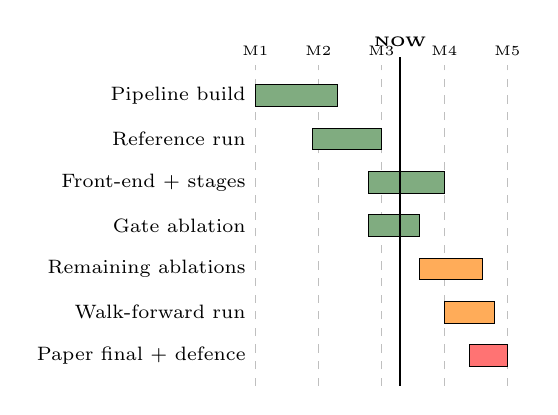
\begin{tikzpicture}[yscale=0.55, xscale=0.8, font=\scriptsize]
  \def\lanex{5.9}
  \foreach \t/\l in {0/M1,1/M2,2/M3,3/M4,4/M5}{
    \draw[gray!50, thin, dashed] (\t,-7.2) -- (\t,0.2);
    \node[above, font=\tiny] at (\t,0.2) {\l};
  }
  \node[anchor=east] at (0,-0.5) {Pipeline build};
  \draw[fill=green!35!black!50!white] (0,-0.75) rectangle (1.3,-0.25);
  \node[anchor=east] at (0,-1.5) {Reference run};
  \draw[fill=green!35!black!50!white] (0.9,-1.75) rectangle (2.0,-1.25);
  \node[anchor=east] at (0,-2.5) {Front-end + stages};
  \draw[fill=green!35!black!50!white] (1.8,-2.75) rectangle (3.0,-2.25);
  \node[anchor=east] at (0,-3.5) {Gate ablation};
  \draw[fill=green!35!black!50!white] (1.8,-3.75) rectangle (2.6,-3.25);
  \node[anchor=east] at (0,-4.5) {Remaining ablations};
  \draw[fill=orange!65!white] (2.6,-4.75) rectangle (3.6,-4.25);
  \node[anchor=east] at (0,-5.5) {Walk-forward run};
  \draw[fill=orange!65!white] (3.0,-5.75) rectangle (3.8,-5.25);
  \node[anchor=east] at (0,-6.5) {Paper final + defence};
  \draw[fill=red!55!white] (3.4,-6.75) rectangle (4.0,-6.25);
  \draw[thick, black] (2.3,-7.2) -- (2.3,0.4) node[above, font=\tiny\bfseries, black]{\textbf{NOW}};
\end{tikzpicture}
\caption{Timeline. Green = complete, orange = in progress, red =
scheduled. The vertical line marks mid-term.}
\label{fig:gantt}
\end{figure}

Milestones M1--M3 are complete. M4 (remaining ablations, walk-forward,
final paper) is active. M5 is the defence and submission window.

%% =====================================================================
\section{Limitations}
\label{sec:limitations}

Four limitations are carried forward to the final milestone:

\emph{Sample size.} $n{=}53$ decisions per ticker. Sharpe comparisons
against baselines do not separate at $\alpha{=}0.05$.

\emph{Universe size.} Four US equities plus one probe. Replication
across sectors and markets is future work; the NEPSE wiring is
already in the code for a cross-market replication.

\emph{Model family.} All measurements are on Gemini 3.5 Flash /
Pro / Flash-lite. Model-family effects are not controlled.

\emph{Paper-trade fees.} US retail fee profile ($\sim$2 bp
round-trip). Market-impact modeling is deferred.

These are the same limitations reported in the companion research
paper; the mid-term framing is that each has a concrete mitigation
scheduled before the final milestone.

%% =====================================================================
\section{Conclusion}

Argos is a measurement-first multi-agent LLM trading research desk.
At the mid-term it ships: a complete pipeline with structured
outputs and per-decision audit, a trader-facing front-end that
pairs raw evidence with each agent's verdict, a 211-decision
reference run, a cost--recall Pareto frontier for the
selective-reasoning gate, per-agent calibration disaggregation,
and a first-draft research paper. Three ablation arms, the
walk-forward out-of-sample run, and the final manuscript revision
remain for the final milestone. The reproducibility story
(pinned model IDs, append-only JSONL journals, git SHA per record,
shared LLM cache) is the project's primary research-integrity
asset and will be preserved through the remaining work.

%% =====================================================================
\begin{thebibliography}{99}\footnotesize

\bibitem{tradingagents}
Y.~Xiao \emph{et al.},
``TradingAgents: Multi-agent LLM financial trading framework,''
\emph{arXiv:2412.20138}, 2024.

\bibitem{finagent}
A.~Zhang \emph{et al.},
``A multimodal foundation agent for financial trading,''
\emph{arXiv:2402.18485}, 2024.

\bibitem{finmem}
Y.~Yu \emph{et al.},
``FinMem: A performance-enhanced LLM trading agent,''
\emph{arXiv:2311.13743}, 2023.

\bibitem{chow1970}
C.~K. Chow,
``On optimum recognition error and reject tradeoff,''
\emph{IEEE Trans.\ Inf.\ Theory}, 1970.

\bibitem{geifman2017selective}
Y.~Geifman and R.~El-Yaniv,
``Selective classification for deep neural networks,''
in \emph{NeurIPS}, 2017.

\bibitem{mozannar2020defer}
H.~Mozannar and D.~Sontag,
``Consistent estimators for learning to defer to an expert,''
in \emph{ICML}, 2020.

\bibitem{du2023debate}
Y.~Du \emph{et al.},
``Improving factuality and reasoning in language models through
multiagent debate,'' \emph{arXiv:2305.14325}, 2023.

\bibitem{liang2023divergent}
T.~Liang \emph{et al.},
``Encouraging divergent thinking in LLMs through multi-agent
debate,'' \emph{arXiv:2305.19118}, 2023.

\bibitem{chen2023frugalgpt}
L.~Chen \emph{et al.},
``FrugalGPT: How to use LLMs while reducing cost and improving
performance,'' \emph{arXiv:2305.05176}, 2023.

\bibitem{ong2024routellm}
I.~Ong \emph{et al.},
``RouteLLM: Learning to route LLMs with preference data,''
\emph{arXiv:2406.18665}, 2024.

\bibitem{langgraph}
LangChain Inc.,
``LangGraph: Building stateful multi-actor LLM applications,''
2024. [Online]. Available:
\url{https://langchain-ai.github.io/langgraph/}

\end{thebibliography}

\end{document}
